\chapter{Introduction}
\section{The BeachBot Project}
The BeachBot project is a focus project at ETH Zurich. During the two last semesters of the bachelor studies, the team had the opportunity to develop a mobile and autonomous robot prototype for creating sand drawings on beaches (the final robot prototype is shown in \autoref{fig:beachbot}). In total 7 mechanical engineering students, one electrical engineering student and two industrial design students (from the Zürcher Hochschule der Künste) were working on the project. 

The result of the project is a 3 wheeled mobile robot that can drive autonomously. The key features are:
\begin{description}
\item[Localization] The robot is able to reliably localize itself on the beach, using a laser range finder and 3 or more reflective poles. An localization accuracy of about 3 centimetres was achieved.
\item[Driving speed and turning radius] The top speed of the robot is about 0.4 metres per second and it can turn on the spot. Both back wheels are independently steerable. The front wheel is also actuated. This is done to reduce the risk of getting stuck in sand.
\item[Rake] The main drawing tool of the robot is a rake. The rake consists of seven pin-pairs which are individually liftable.
\item[Controller] The controller uses the output from the localization to steer the robot so that it follows a pre-defined trajectory.
\item[Automatic Path Generation] An application was created to generate the trajectory for an arbitrary input drawing, that can then be drawn on the beach.
\end{description}

The robot was tested successfully at the beach.

\begin{figure}
\centering
\begin{subfigure}[c]{1\textwidth}
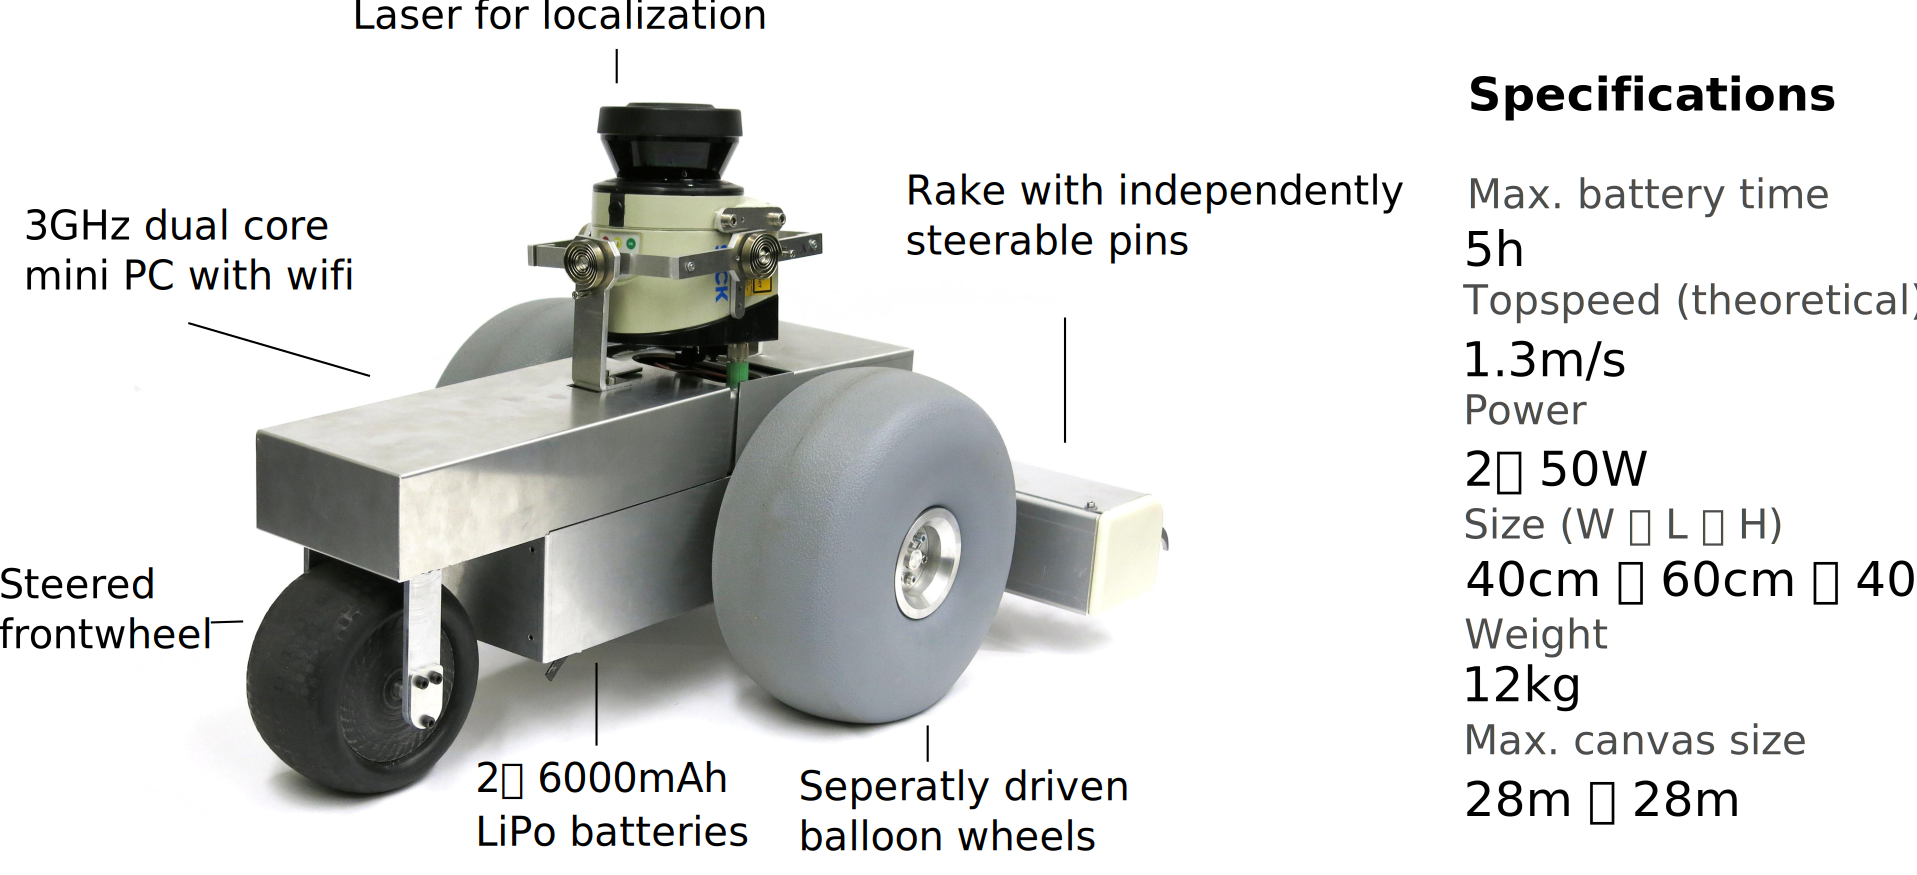
\includegraphics[width=\textwidth]{images/introduction/beachbot_spec.pdf} 
\end{subfigure}
\\
\begin{subfigure}[c]{1\textwidth}
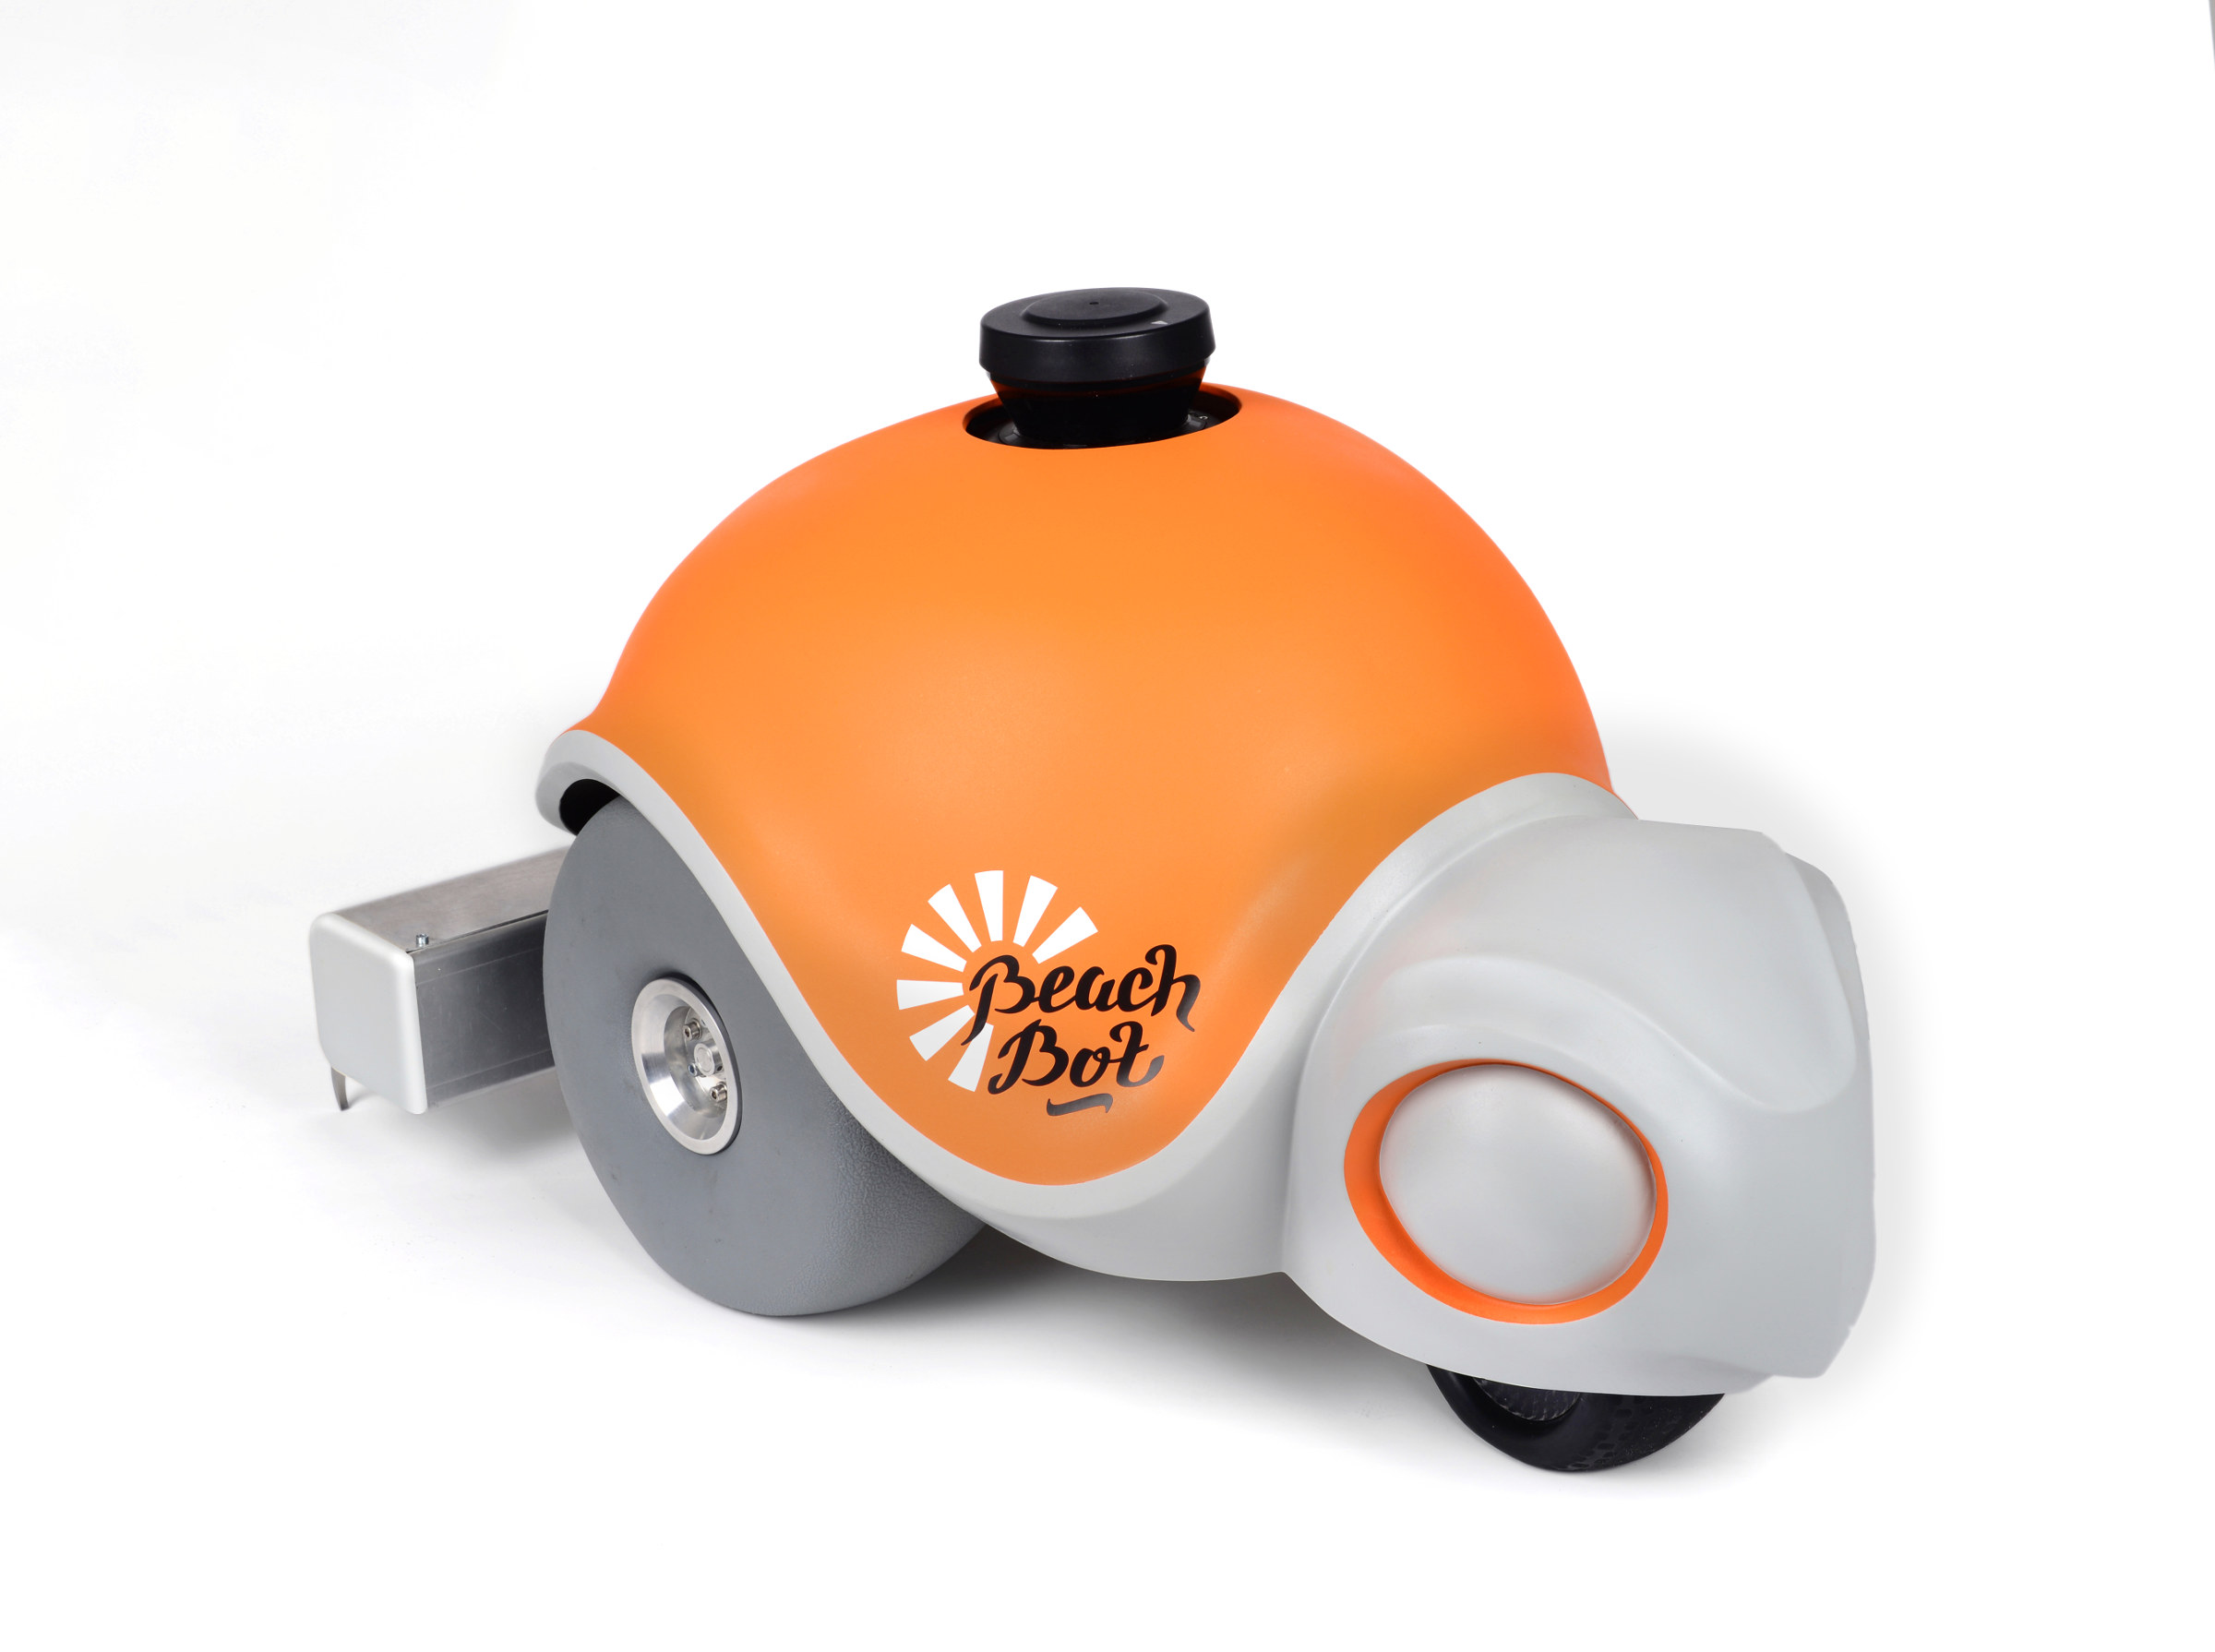
\includegraphics[width=\textwidth]{images/introduction/final_shell_scaled_down.jpg} 
\caption{The outer shell of the BeachBot}
\end{subfigure}
\\
\vspace{2cm}
\begin{subfigure}[c]{0.46\textwidth}
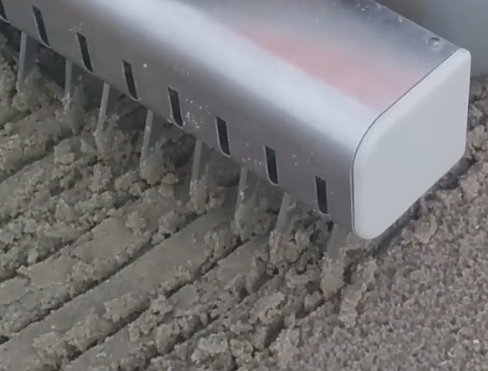
\includegraphics[width=\textwidth]{images/introduction/localization_precision.png} 
\caption{The rake in action}
\end{subfigure}
~~
\begin{subfigure}[c]{0.3\textwidth}
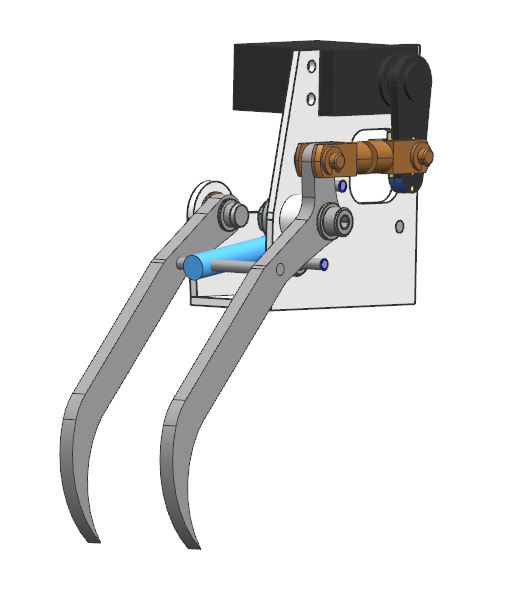
\includegraphics[width=\textwidth]{images/introduction/rake_pins.png}
\caption{One rake unit with servo motor and pin pair.}
\end{subfigure}
\caption{Various images of the BeachBot}
\label{fig:beachbot}
\end{figure} 
